% Results and Discussion

\chapter{Results and Discussion} % Main chapter title

\label{Chapter3} % Change X to a consecutive number; for referencing this chapter elsewhere, use \ref{ChapterX}

%----------------------------------------------------------------------------------------
%	SECTION 1
%----------------------------------------------------------------------------------------

\section{Offline Gait Analysis}

%-----------------------------------
%	SUBSECTION 1
%-----------------------------------
\subsection{Event Detection}

\begin{figure}[th]
\captionsetup{justification=raggedright,singlelinecheck=false}
\centering
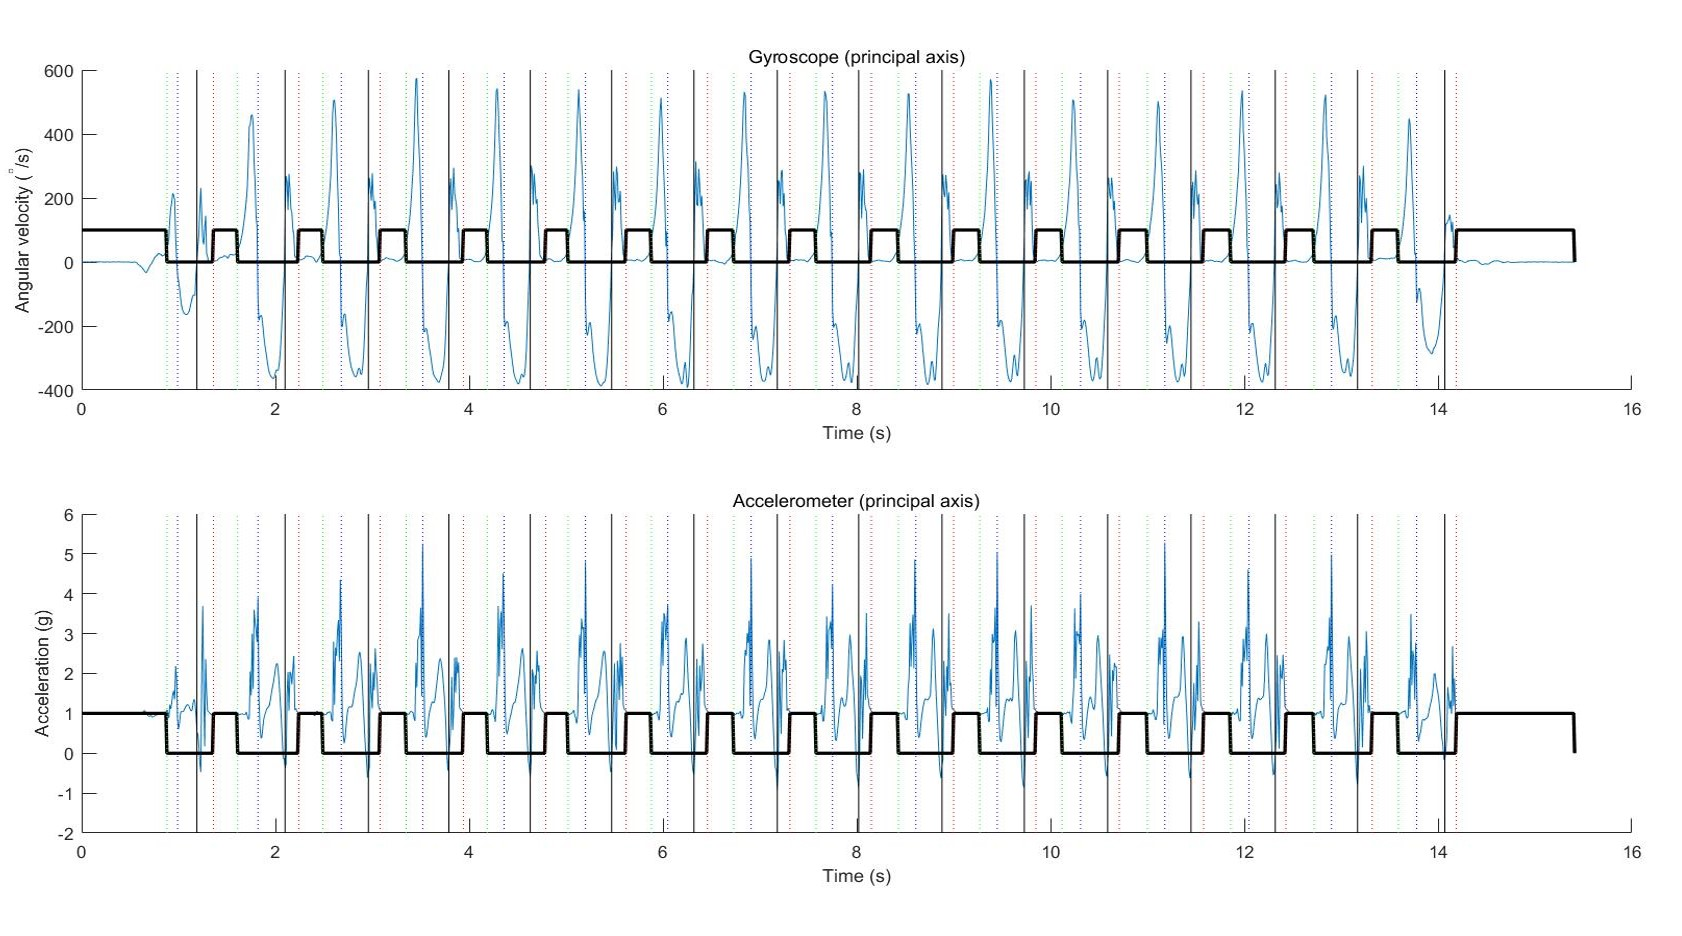
\includegraphics[width=\textwidth,height=\textheight,keepaspectratio]{Figures/gait_event_detection_results.jpg}
\decoRule
\caption[Gait event detection results]{Gait event detection for a sample walking session. Color-coded vertical lines indicate gait events (black: heel-strike, red: foot-flat, green: heel-off, blue: toe-off). Thick black line represents stationary state with zero being stationary.}
\label{fig:gait_event_detection_results}
\end{figure}
\noindent
FSM described in Chapter 2 was used to generate results shown in Figure \ref{fig:gait_event_detection_results}. Gait events were successfully recognized. Gait event detection was only used as a reference and was not required for WIP technique described in this paper.

\newpage
%-----------------------------------
%	SUBSECTION 2
%-----------------------------------
\subsection{Trajectory}

\begin{figure}[th]
%\captionsetup{justification=raggedright,singlelinecheck=false,format=hang}
\captionsetup{justification=raggedright,singlelinecheck=false}
\centering
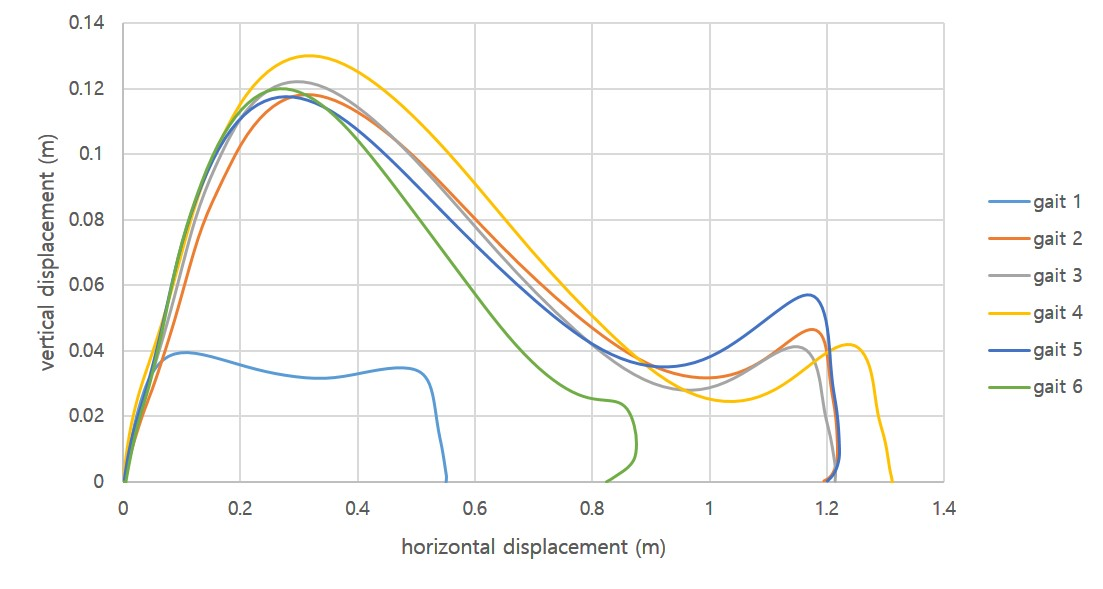
\includegraphics[width=\textwidth,height=\textheight,keepaspectratio]{Figures/gait_feature_extraction_results.jpg}
\decoRule
\caption[Gait feature extraction results]{Gait trajectory for a sample walking session. Gait 1 and 6 are stating and stopping gait sequences, respectively and the rest are steady state gait sequences. Similar results were obtained when compared with \cite{Kit16}.}
\label{fig:gait_feature_extraction_results}
\end{figure}
\noindent
Kitagawa's method summarized in Chapter 2 was used obtain gait trajectory shown in Figure \ref{fig:gait_feature_extraction_results}. Time derivative of the horizontal and vertical component of the trajectory yields $V_{r}$ and $V_{z}$. Period $T$ can also be determined from the results. These parameters provide a baseline for the $scale factor$.

\newpage
%----------------------------------------------------------------------------------------
%	SECTION 2
%----------------------------------------------------------------------------------------

\section{Locomotion Generation}

%-----------------------------------
%	SUBSECTION 1
%-----------------------------------
\subsection{WIP Event Detection}

\begin{figure}[th]
\captionsetup{justification=raggedright,singlelinecheck=false}
\centering
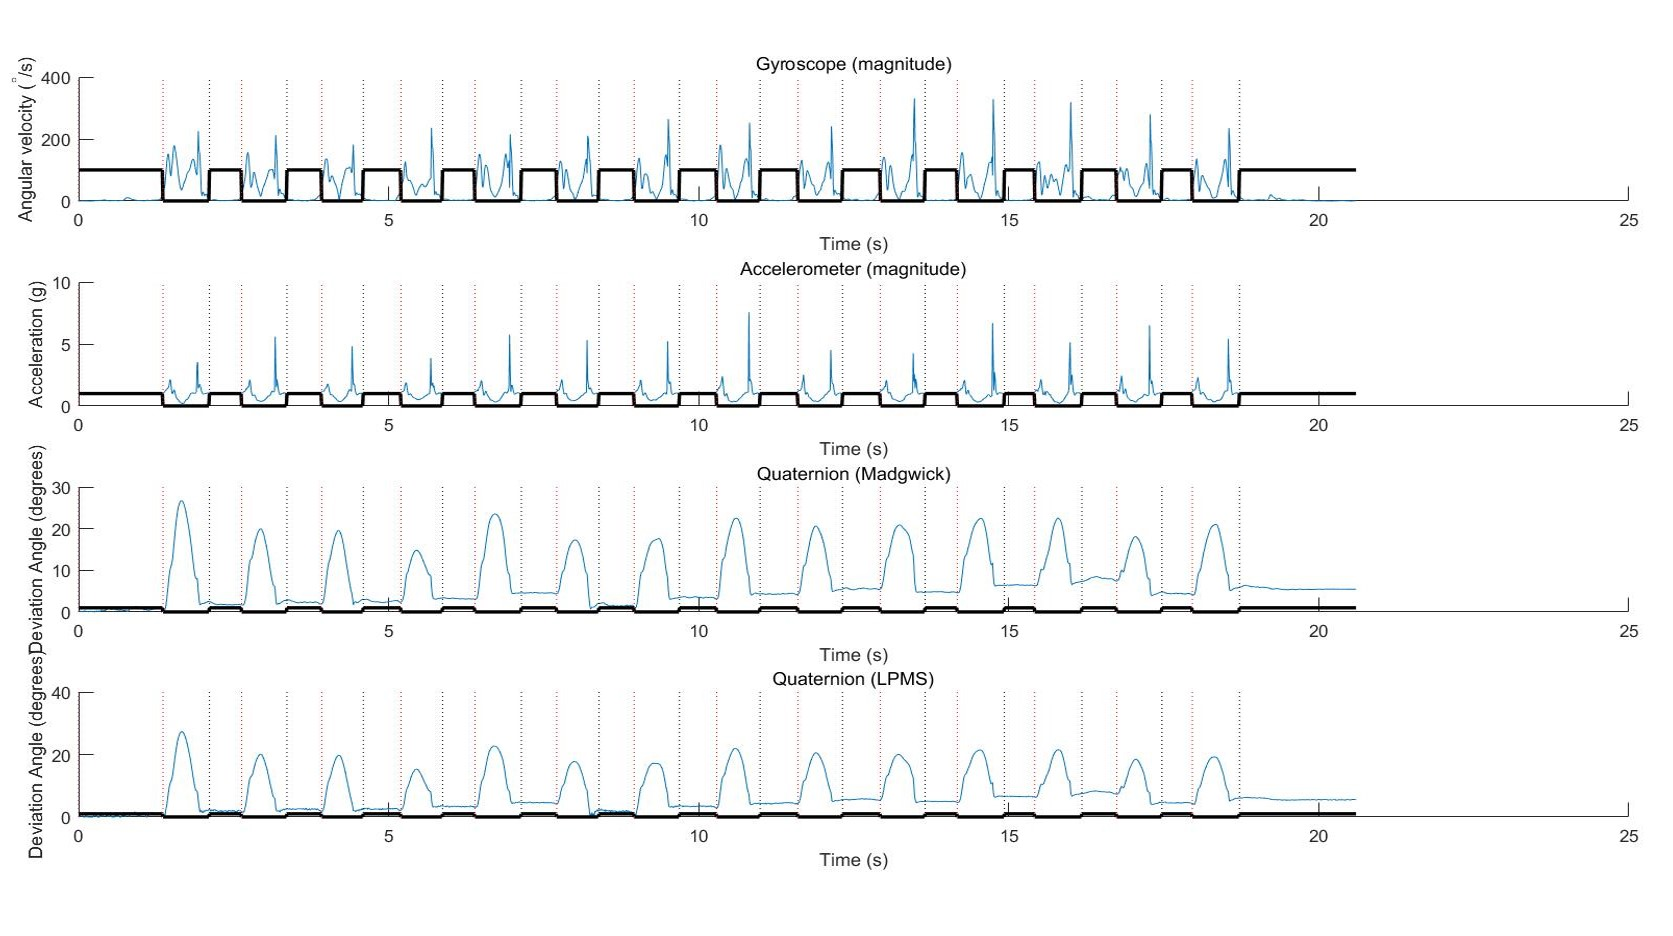
\includegraphics[width=\textwidth,height=\textheight,keepaspectratio]{Figures/wip_event_detection.jpg}
\decoRule
\caption[WIP event detection results]{WIP event detection for a sample WIP session. Color-coded vertical lines indicate state transition (black: foot-strike, red: foot-off). Thick black lines represent stationary state with zero being stationary.}
\label{fig:wip_event_detection}
\end{figure}
\noindent
WIP event detection is shown in Figure \ref{fig:wip_event_detection}. Stationary state is determined by a FSM described in Chapter 2, with simple thresholding for state transition. Deviation angles shown in Figure \ref{fig:wip_event_detection} are derived from axis-angle representation of relative quaternions to initial orientation. In order to verify Madgwick's algorithm, it was compared against quaternion readings from the LPMS-B2 IMU sensor.
\\\\
Figure \ref{fig:wip_quaternion_decomposition} overlays WIP events with xy (pitch and roll) and z (yaw) components of deviation angle. xy component $\phi_{xy}$ and z component $\phi_{z}$ can be obtained from relative quaternion to initial orientation $q = [q_{0},   q_{1},   q_{2},   q_{3}]$ with the following equation.
\\\\
\centerline{$\phi_{z} = 2atan2(q_{3},   q_{0})$ \indent $-\pi\leq \phi_{z}\leq\pi$}
\\\\
\centerline{$\phi_{xy} = 2acos\Big(\dfrac{q_{0}}{cos(\phi_{z}/2)}\Big)$\indent or\indent $2acos\Big(\dfrac{q_{3}}{sin(\phi_{z}/2)}\Big)$ \indent $-\pi\leq \phi_{xy}\leq\pi$}
\\\\
As shown in Figure \ref{fig:wip_quaternion_decomposition}, xy component of deviation angle (in yellow) starts rising right after foot-off event but settles slightly before foot-strike event, suggesting a slight lag in the foot-strike event detection. This is due to use of filtered values for thresholding in the stationary FSM as mentioned in Chapter 2. By adopting xy component of deviation angle as a means of detecting foot-strike event, lag can be reduced at the expense of added complexity of the FSM. However, for the purpose of implementing the WIP technique, slight lag is encouraged to prevent unintended stops in the generated locomotion. Thus, a simple thresholding of filtered acceleration and angular velocity is used for stationary FSM.

\newpage

\begin{figure}[th]
\captionsetup{justification=raggedright,singlelinecheck=false}
\centering
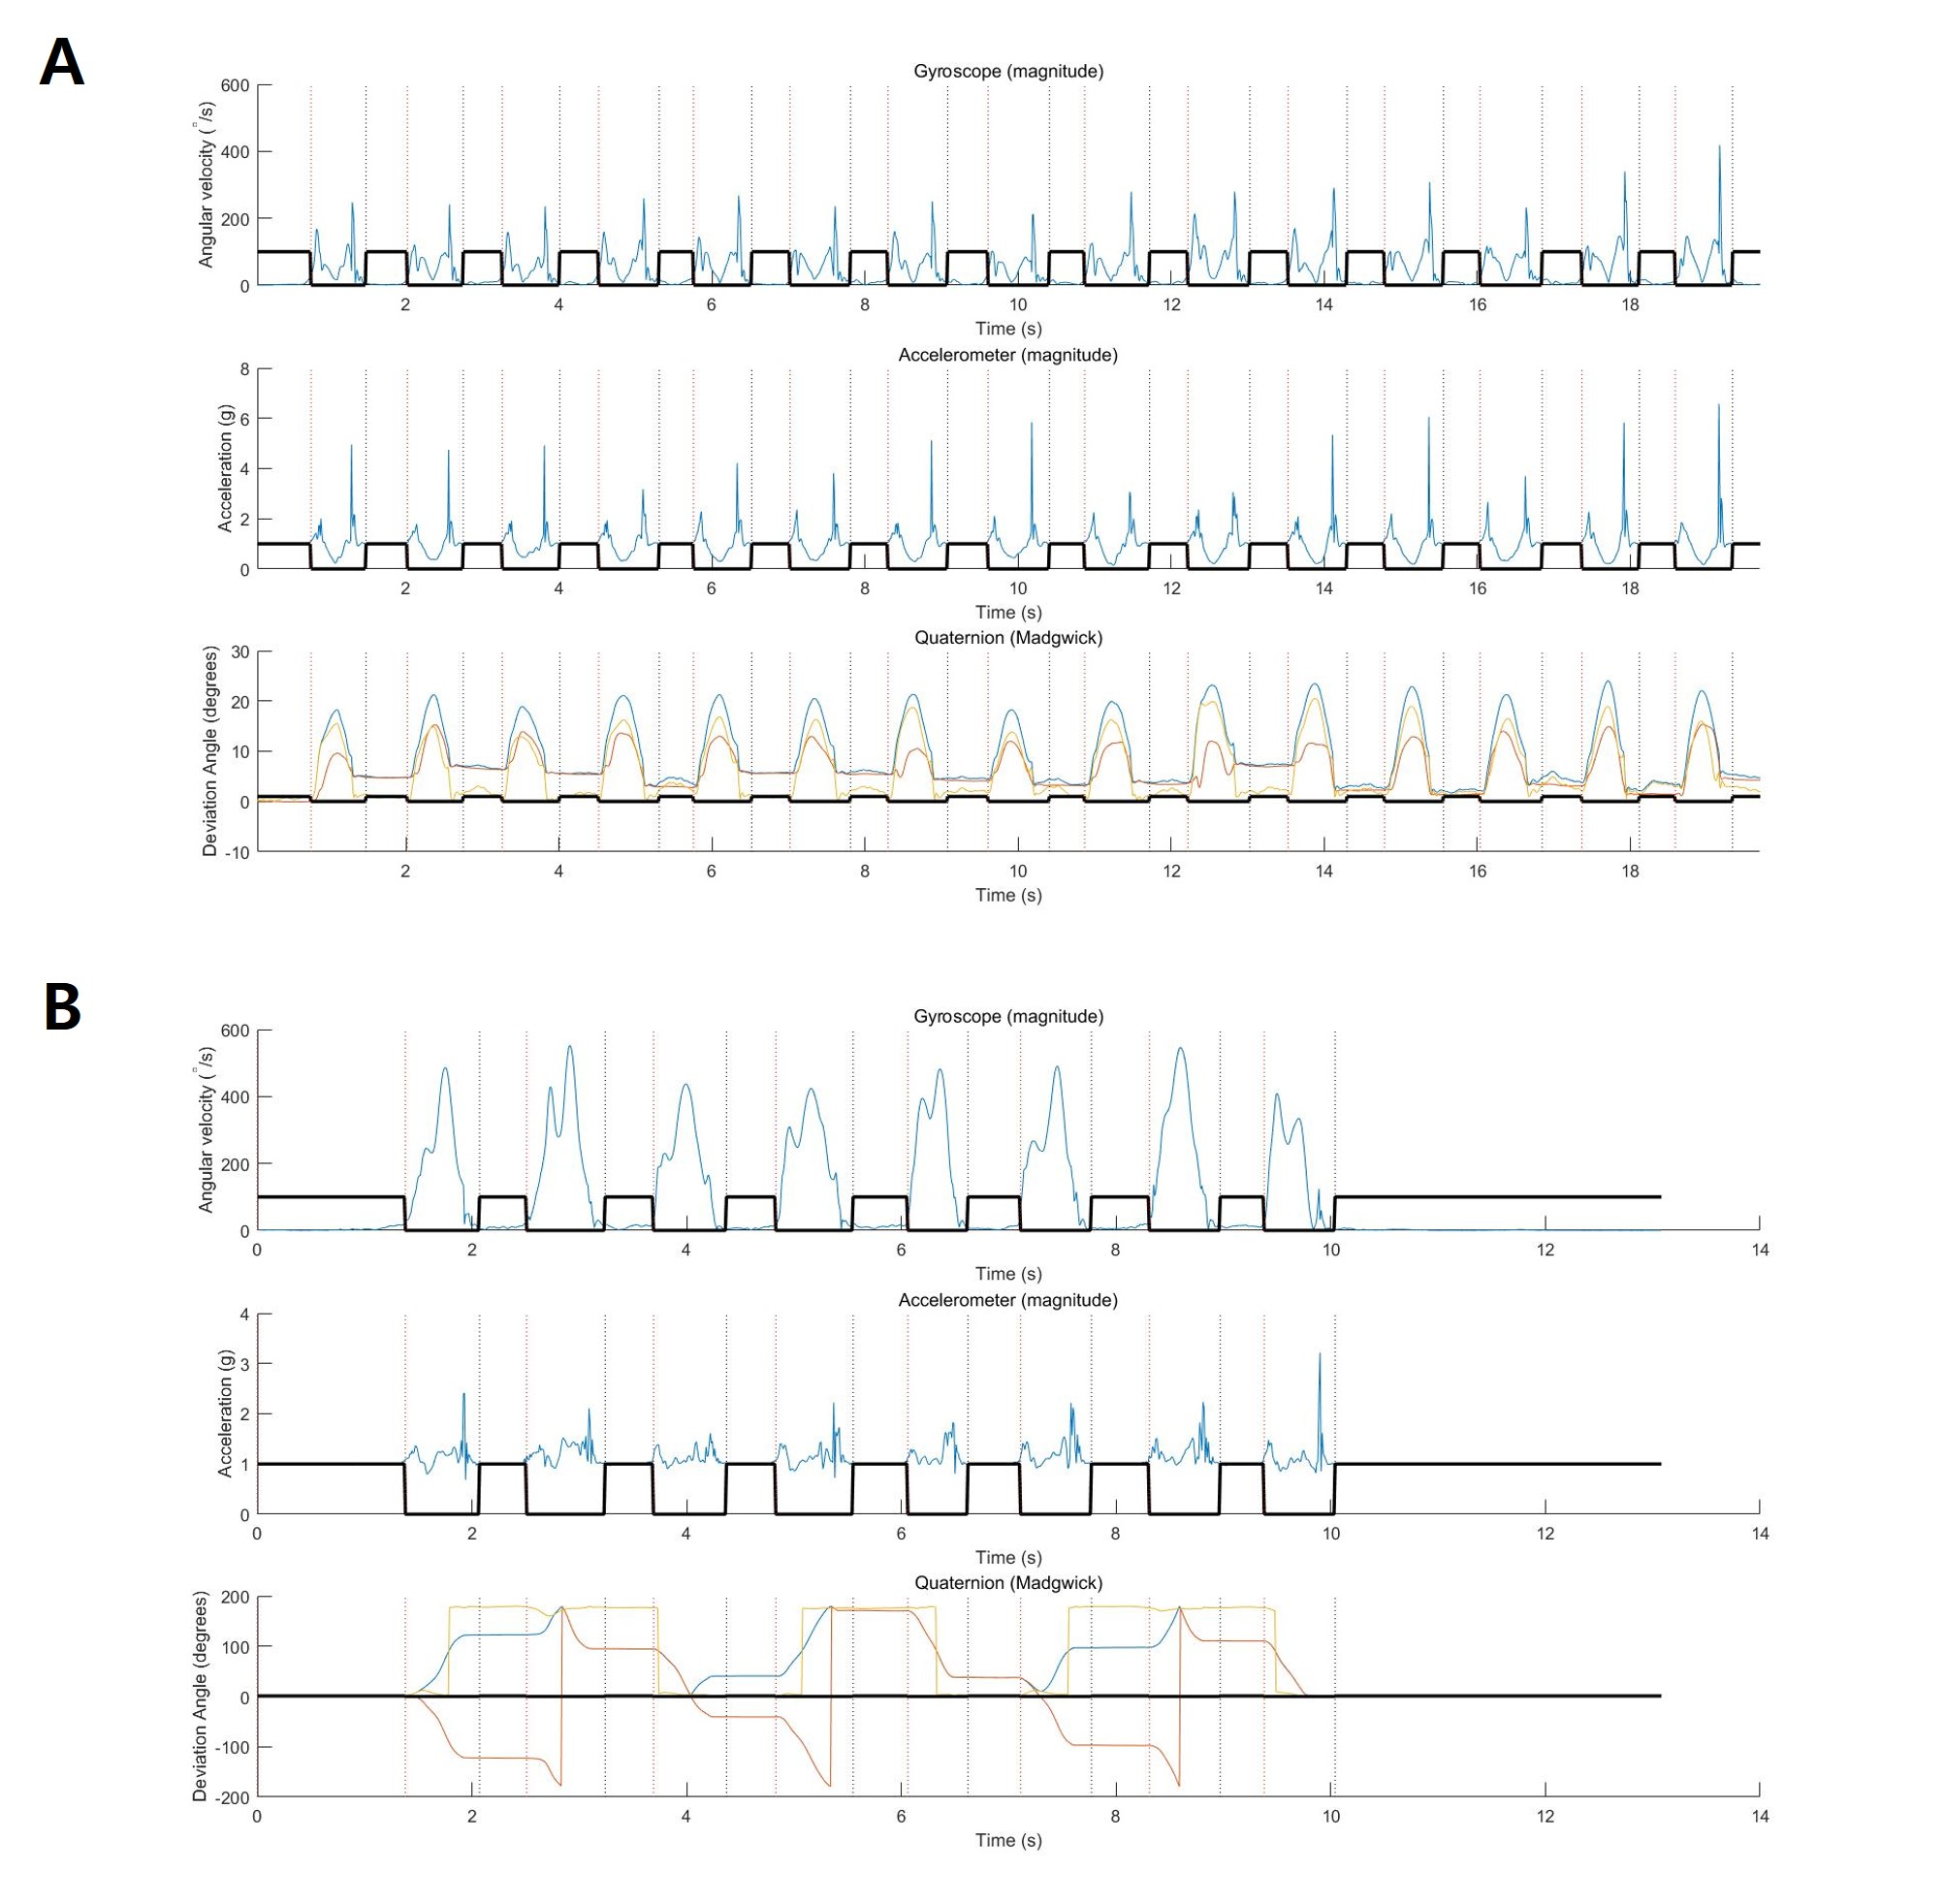
\includegraphics[width=\textwidth,height=\textheight,keepaspectratio]{Figures/wip_quaternion_decomposition.jpg}
\decoRule
\caption[WIP event detection with quaternion decomposition]{WIP event detection for A. simple WIP motion, B. WIP motion with rotation. Color-coded vertical lines indicate state transition (black: foot-strike, red: foot-off). Thick black lines represent stationary state with zero being stationary. Angles obtained from axis-angle representation of the relative quaternions to initial orientation can be decomposed into xy and z component as shown in the third row of A and B (blue: combined, red: z component, yellow: xy component).}
\label{fig:wip_quaternion_decomposition}
\end{figure}
\noindent

%-----------------------------------
%	SUBSECTION 2
%-----------------------------------
\subsection{WIP Sessions}

Direct and indirect approach for locomotion generation was conducted on four different WIP sessions - natural WIP, leisurely WIP, marching WIP and natural WIP with rotation. With offline analysis of gait, the $scale factor$ was appropriately set to generate locomotion that is similar to that of walking. The results are presented in Figure \ref{fig:wip_session1} through \ref{fig:wip_session4}. From the figures it can be seen that the indirect approach maintains identical starting and stopping latencies with the added benefit of reduced jerkiness and the detection of rotation-in-place as seen in Figure \ref{fig:wip_session4}. Demonstration of proposed WIP technique is shown in Figure \ref{fig:demo}.

\begin{figure}[th]
\captionsetup{justification=raggedright,singlelinecheck=false}
\centering
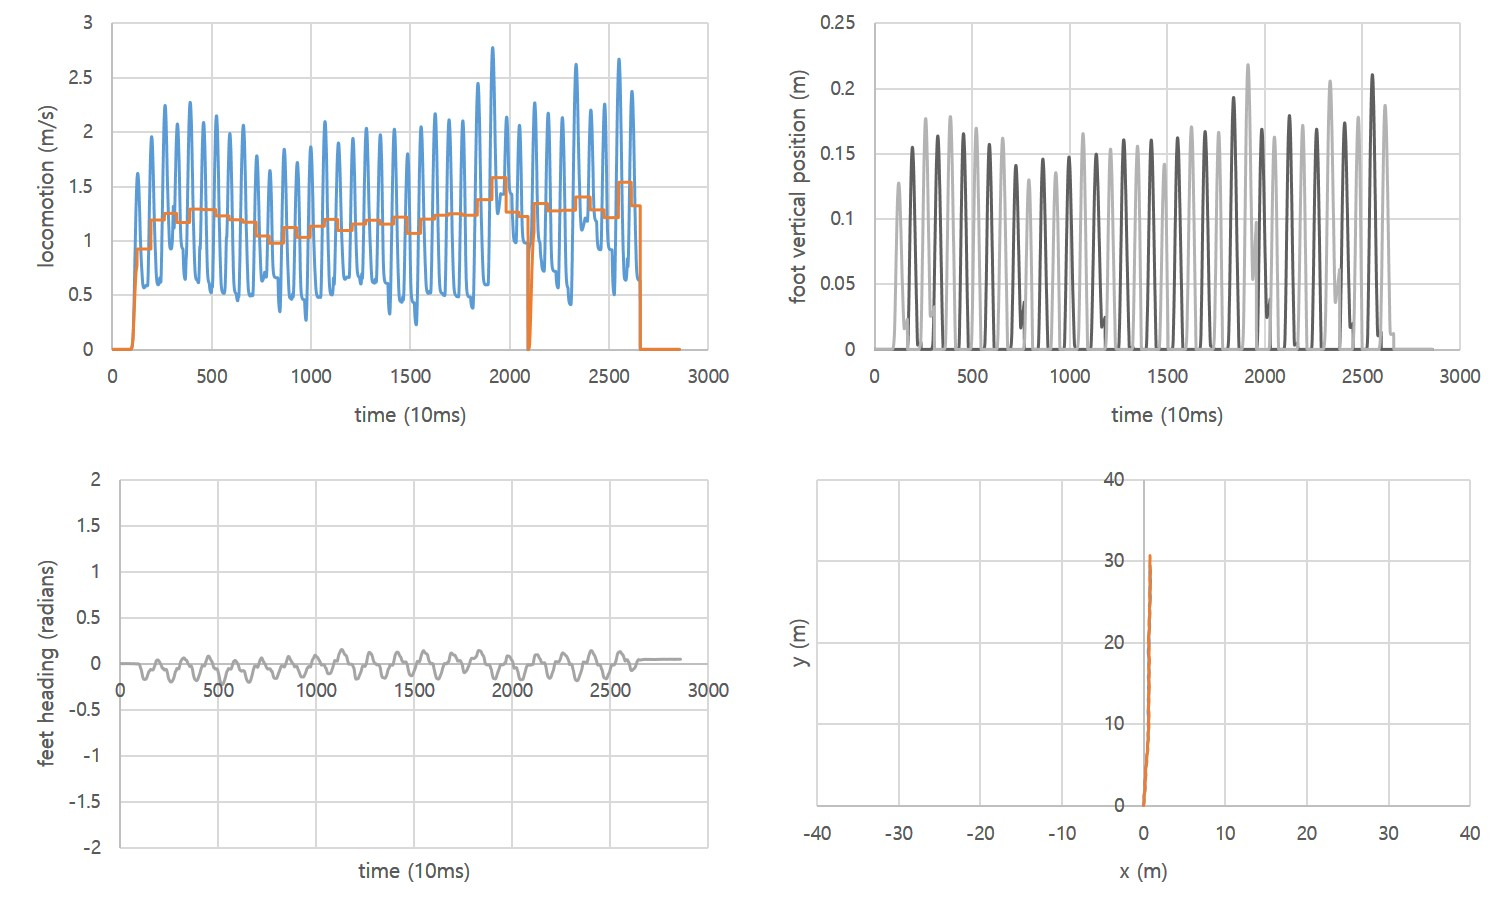
\includegraphics[width=\textwidth,height=\textheight,keepaspectratio]{Figures/session1.jpg}
\decoRule
\caption[WIP session 1]{Locomotion generation for WIP session 1 (natural WIP, medium amplitude). Direct approach is in blue and indirect approach is in orange. Left foot and right foot is in black and grey, respectively.}
\label{fig:wip_session1}
\end{figure}

\begin{figure}[th]
\captionsetup{justification=raggedright,singlelinecheck=false}
\centering
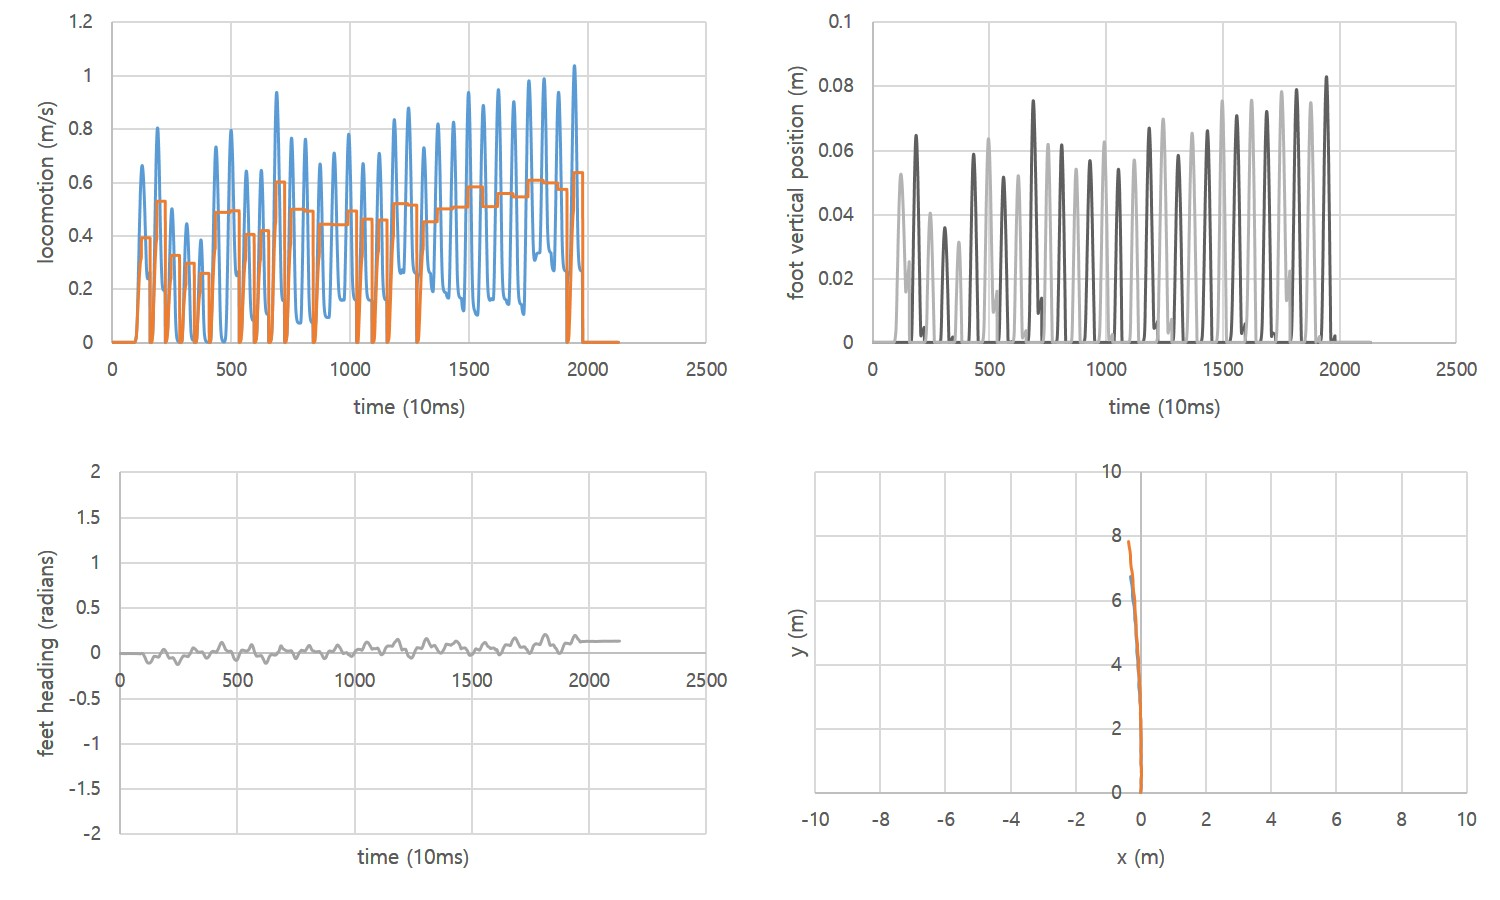
\includegraphics[width=\textwidth,height=\textheight,keepaspectratio]{Figures/session2.jpg}
\decoRule
\caption[WIP session 2]{Locomotion generation for WIP session 2 (leisurely WIP, small amplitude). Direct approach is in blue and indirect approach is in orange. Left foot and right foot is in black and grey, respectively.}
\label{fig:wip_session2}
\end{figure}

\begin{figure}[th]
\captionsetup{justification=raggedright,singlelinecheck=false}
\centering
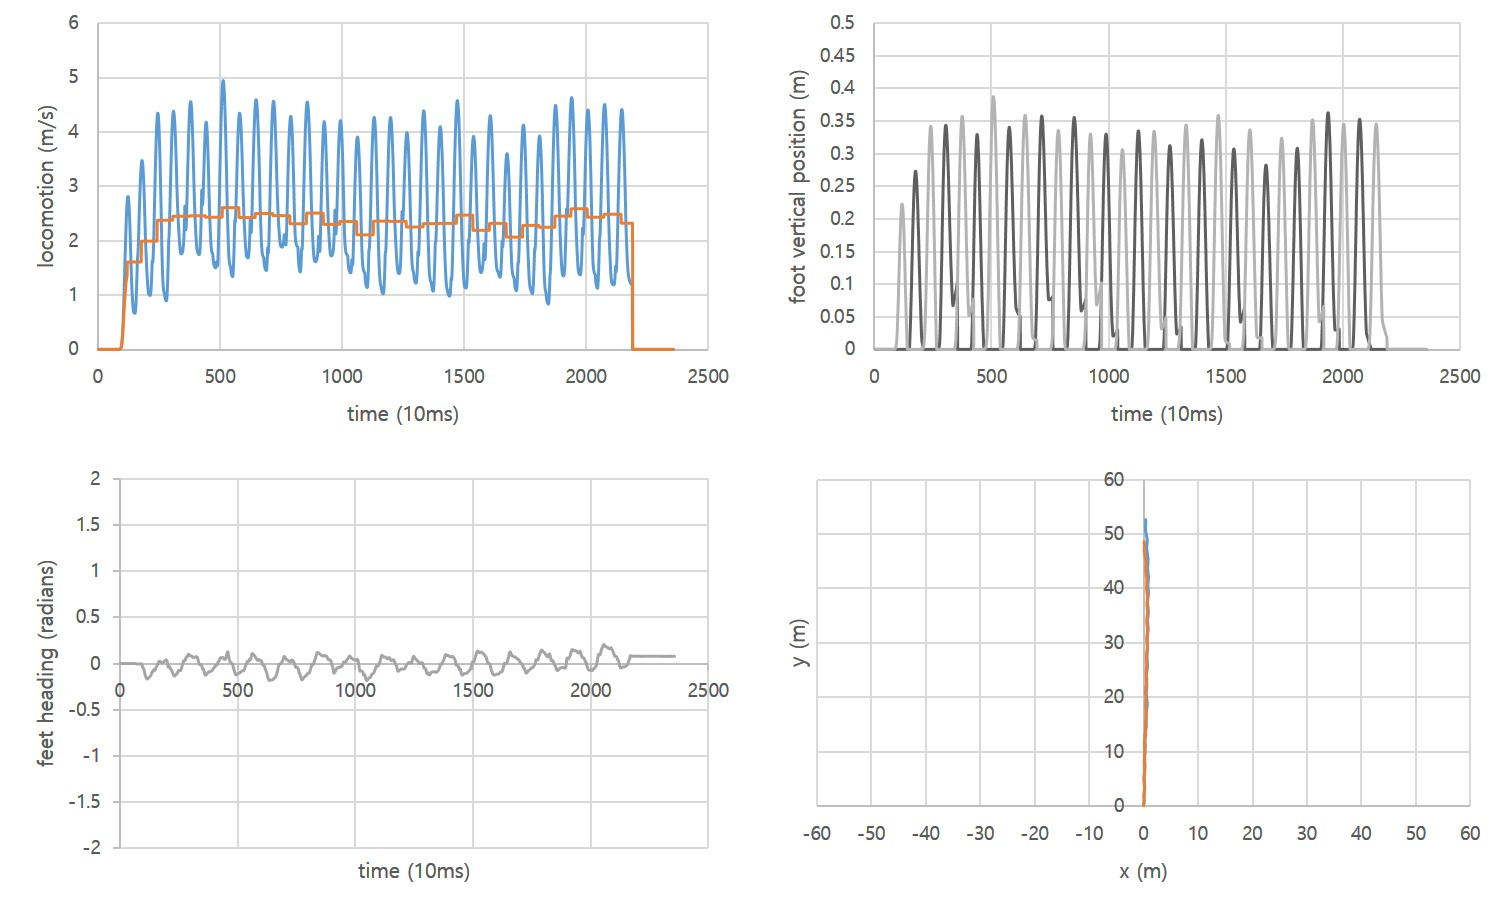
\includegraphics[width=\textwidth,height=\textheight,keepaspectratio]{Figures/session3.jpg}
\decoRule
\caption[WIP session 3]{Locomotion generation for WIP session 3 (marching WIP, large amplitude). Direct approach is in blue and indirect approach is in orange. Left foot and right foot is in black and grey, respectively.}
\label{fig:wip_session3}
\end{figure}

\begin{figure}[th]
\captionsetup{justification=raggedright,singlelinecheck=false}
\centering
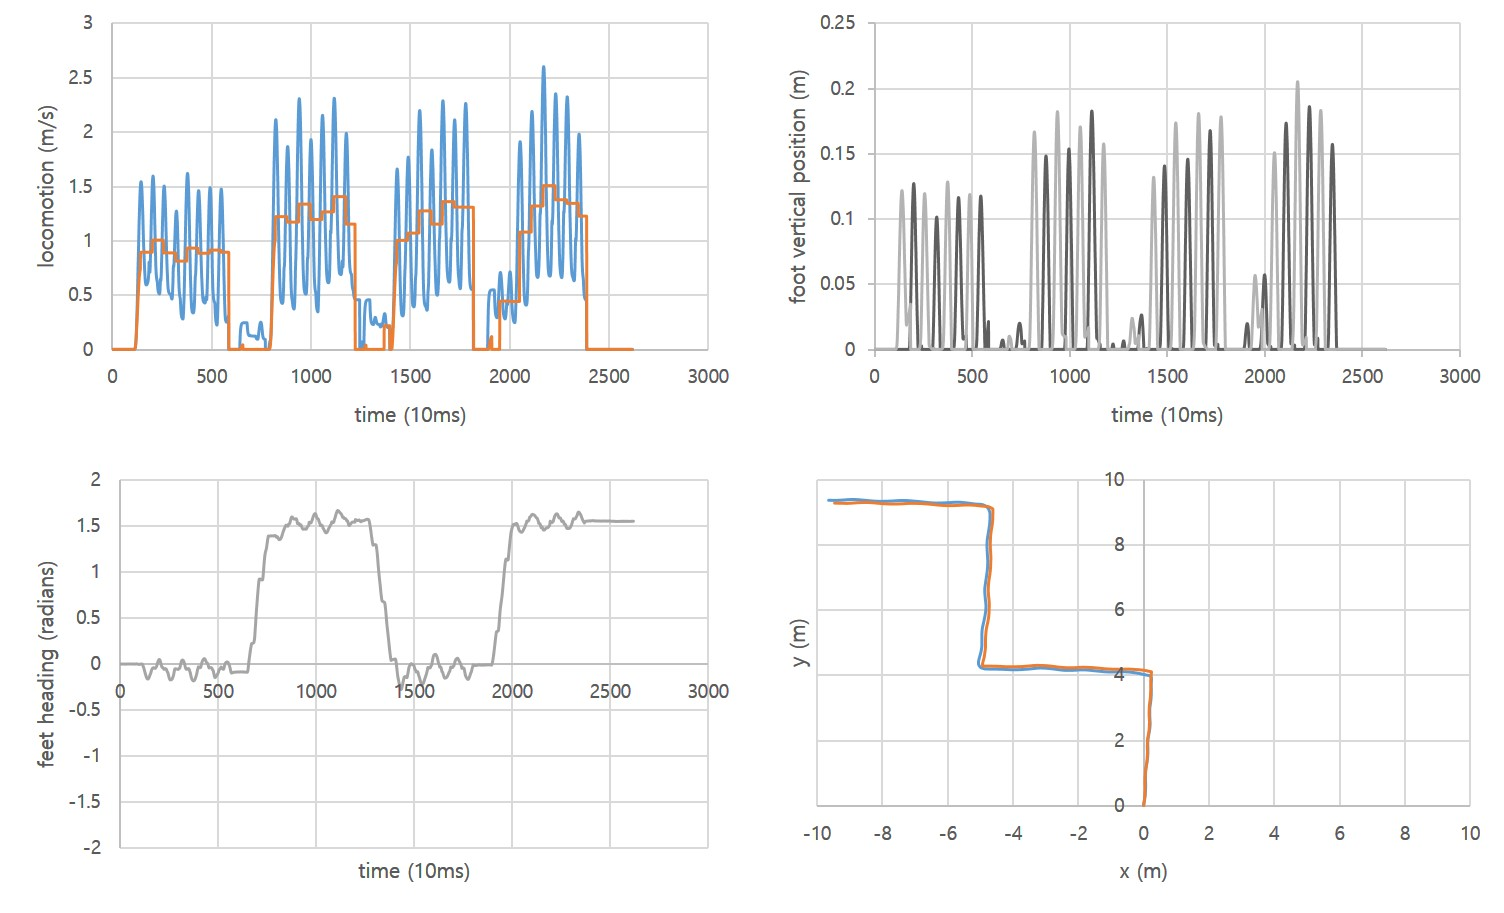
\includegraphics[width=\textwidth,height=\textheight,keepaspectratio]{Figures/session4.jpg}
\decoRule
\caption[WIP session 4]{Locomotion generation for WIP session 4 (natural WIP with rotation). Direct approach is in blue and indirect approach is in orange. Left foot and right foot is in black and grey, respectively.}
\label{fig:wip_session4}
\end{figure}

\begin{figure}[th]
\captionsetup{justification=raggedright,singlelinecheck=false}
\centering
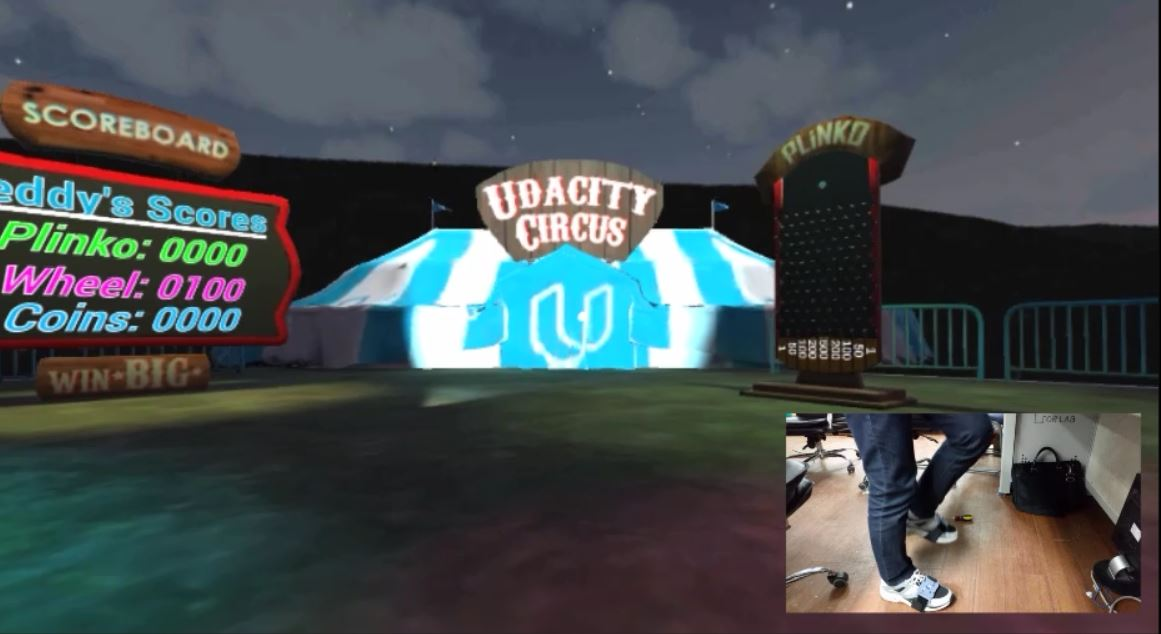
\includegraphics[width=\textwidth,height=\textheight,keepaspectratio]{Figures/demo.jpg}
\decoRule
\caption[Demo]{Demonstration of proposed WIP technique with Unity (sample scene from Udacity)}
\label{fig:demo}
\end{figure}